\begin{figure}
\centering
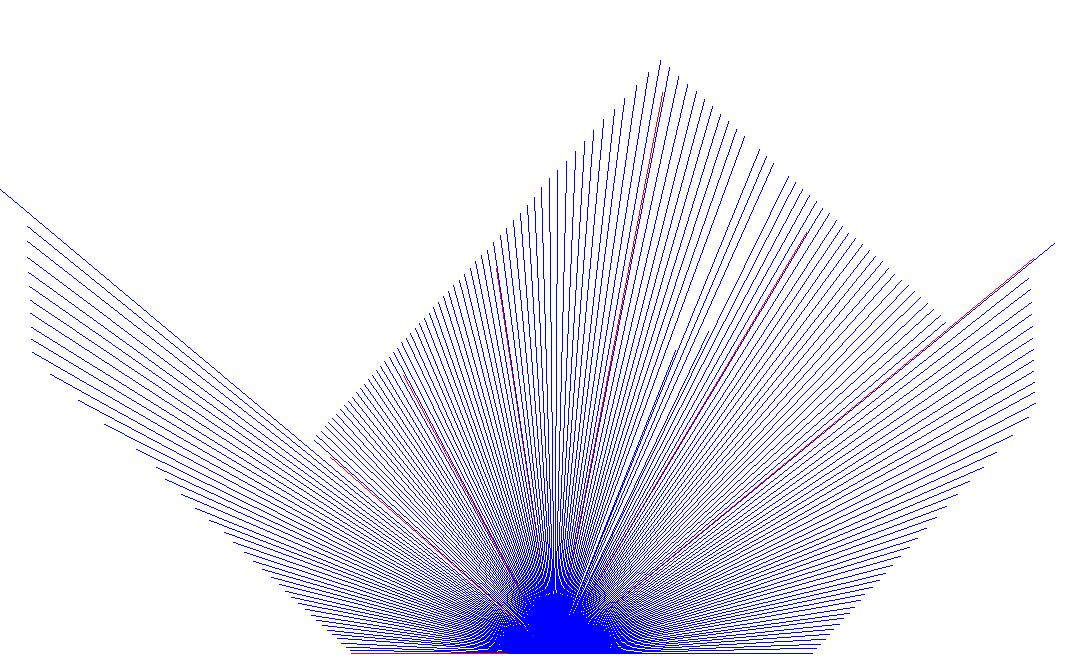
\includegraphics[width=.7\textwidth]{Sensor.jpg}
\caption{The data from the laser range scanner and the sonar, as represented by
our program. Red represents sonar data, blue represents laser data.}
\label{fig:sonarLaserData}
\end{figure}

The sensor module has two tasks. The first task is forwarding different kind of 
sensor messages to the mapper module and the reflex module. The second task is to
display the sonar and range scanner (laser) sensor data graphically. This allows 
to see if the data is correctly parsed by the coordinator module and received by 
this module with one quick glance. Furthermore it can be used for other debug 
purposes, such as checking correct reflex behavior. See figure \ref{fig:sonarLaserData}
for an example of displayed sensor data. 


